\documentclass{article}

\usepackage{amsmath,amssymb,bm}
\usepackage{tnptimes}
\usepackage{graphicx}
\graphicspath{{figures/}}
\usepackage{subfig}

\title{Variance of Stepwise Sample Means}
\author{Jingxuan Yang%
\thanks{Jingxuan Yang is with the Department of Automation, Tsinghua University, Beijing 100084, China (email: yangjx20@mails.tsinghua.edu.cn).}
}

\begin{document}

\maketitle

In this note, we will analyze the variance of stepwise sample means.

Suppose the data samples are $\{x_i\}_{i=1}^n$. The sample mean is
\begin{equation}
  \bar{x}_n=\frac{1}{n}\sum_{i=1}^nx_i.
\end{equation}
The sample variance is
\begin{equation}
  \label{eq:var_def}
  \sigma_n^2
  =\frac{1}{n}\sum_{i=1}^n(x_i-\bar{x}_n)^2
  =\frac{1}{n}\sum_{i=1}^nx_i^2-\bar{x}_n^2.
\end{equation}
Therefore, the matrix form of sample variance is
\begin{equation}
  \begin{aligned}
    \sigma_n^2
    &=\frac{1}{n}(x_1^2+\cdots+x_n^2)-\frac{1}{n^2}(x_1+\cdots+x_n)^2\\
    &=\frac{1}{n^2}x^\top\begin{bmatrix}
      n & & & \\
      & n & & \\
      & & \ddots & \\
      & & & n \\
    \end{bmatrix}x
    -\frac{1}{n^2}x^\top\begin{bmatrix}
      1 & 1 & \cdots & 1 \\
      1 & 1 & \cdots & 1 \\
      \vdots & \vdots & \ddots & \vdots \\
      1 & 1 & \cdots & 1 \\
    \end{bmatrix}x \\
    &=\frac{1}{n^2}x^\top\begin{bmatrix}
      n-1 & -1 & \cdots & -1 \\
      -1 & n-1 & \cdots & -1 \\
      \vdots & \vdots & \ddots & \vdots \\
      -1 & -1 & \cdots & n-1 \\
    \end{bmatrix}x\\
    &\triangleq\frac{1}{n^2}x^\top Vx,\\
  \end{aligned}
\end{equation}
where $V$ is defined as the variance matrix of the sample mean. It's a zero-sum matrix, i.e., the sum of all elements equals zero.

Denote the mean of stepwise sample means $\{\bar{x}_j\}_{j=1}^n$ as
\begin{equation}
    \bar{\bar{x}}_n
    =\frac{1}{n}\sum_{j=1}^n\bar{x}_j
    =\frac{1}{n}\sum_{j=1}^n\frac{1}{j}\sum_{i=1}^jx_i
    =\frac{1}{n}\sum_{i=1}^n\sum_{j=i}^n\frac{1}{j}x_i
    =\frac{1}{n}\sum_{i=1}^n\gamma_{i,n} x_i,
\end{equation}
where
\begin{equation}
  \gamma_{i,n}\triangleq\sum_{j=i}^n\frac{1}{j},\quad
  \frac{1}{n}\sum_{i=1}^n\gamma_{i,n}=1,
\end{equation}
and the variance of stepwise sample means as
\begin{equation}
  \bar{\sigma}_n^2
  =\frac{1}{n}\sum_{i=1}^n(\bar{x}_i-\bar{\bar{x}}_n)^2=\frac{1}{n}\sum_{i=1}^n\bar{x}_i^2-\bar{\bar{x}}_n^2,
\end{equation}
which is actually the variance of the mean of stepwise sample means. There are two mean operations here, and thus this variance is usually less than the sample variance.

The matrix form of this variance is
\begin{equation}
  \begin{aligned}
    \bar{\sigma}_n^2
    &=\frac{1}{n}\left[x_1^2+\left(\frac{x_1+x_2}{2}\right)^2+\cdots+\left(\frac{x_1+\cdots+x_n}{n}\right)^2\right] - \frac{1}{n^2}\left(\sum_{i=1}^n\gamma_{i,n}x_i\right)^2\\
    &=\frac{1}{n^2}x^\top\begin{bmatrix}
      n\xi_{1,n} & n\xi_{2,n} & \cdots & n\xi_{n,n} \\
      n\xi_{2,n} & n\xi_{2,n} & \cdots & n\xi_{n,n} \\
      \vdots & \vdots & \ddots & \vdots \\
      n\xi_{n,n} & n\xi_{n,n} & \cdots & n\xi_{n,n} \\
    \end{bmatrix}x\\
    &\quad
    -\frac{1}{n^2}x^\top\begin{bmatrix}
      \gamma_{1,n}^2 & \gamma_{1,n}\gamma_{2,n} & \cdots & \gamma_{1,n}\gamma_{n,n} \\
      \gamma_{2,n}\gamma_{1,n} & \gamma_{2,n}^2 & \cdots & \gamma_{2,n}\gamma_{n,n} \\
      \vdots & \vdots & \ddots & \vdots \\
      \gamma_{n,n}\gamma_{1,n} & \gamma_{n,n}\gamma_{2,n} & \cdots & \gamma_{n,n}^2 \\
    \end{bmatrix}x\\
    &=\frac{1}{n^2}x^\top\begin{bmatrix}
      n\xi_{1,n}-\gamma_{1,n}^2 & n\xi_{2,n}-\gamma_{1,n}\gamma_{2,n} & \cdots & n\xi_{n,n}-\gamma_{1,n}\gamma_{n,n} \\
      n\xi_{2,n}-\gamma_{2,n}\gamma_{1,n} & n\xi_{2,n}-\gamma_{2,n}^2 & \cdots & n\xi_{n,n}-\gamma_{2,n}\gamma_{n,n} \\
      \vdots & \vdots & \ddots & \vdots \\
      n\xi_{n,n}-\gamma_{n,n}\gamma_{1,n} & n\xi_{n,n}-\gamma_{n,n}\gamma_{2,n} & \cdots & n\xi_{n,n}-\gamma_{n,n}^2 \\
    \end{bmatrix}x\\
    &\triangleq\frac{1}{n^2}x^\top\bar{V}x,
  \end{aligned}
\end{equation}
where $\xi_{i,n}\triangleq\sum_{j=i}^n\frac{1}{j^2}$, and $\bar{V}$ is the variance matrix of the stepwise sample means.
% \begin{equation}
%   \xi_{i,n}\triangleq\sum_{j=i}^n\frac{1}{j^2}.
% \end{equation}

Taking the first element of $\bar{V}$ as an example, it can be expressed as
\begin{equation}
  \begin{aligned}
    n\xi_{1,n}-\gamma_{1,n}^2
    &=n\sum_{j=1}^n\frac{1}{j^2}-\left(\sum_{j=1}^n\frac{1}{j}\right)^2\\
    &=n\left(1+\frac{1}{2^2}+\cdots\frac{1}{n^2}\right)-\left(1+\frac{1}{2}+\cdots+\frac{1}{n}\right)^2\\
    % &=n-\gamma_{1,n}+\frac{1}{2}\left(\frac{1}{2}n-\gamma_{1,n}\right)+\cdots+\frac{1}{n}(1-\gamma_{1,n})\\
    % &=(n-1)\xi_{1,n}-2\sum_{i\neq j}\frac{1}{ij}\\
    &\to n\frac{\pi^2}{6}-(\ln n+\gamma)^2,\quad n\to\infty,\\
  \end{aligned}
\end{equation}
where $\gamma\approx0.5772$ is the Euler number. It can be found that this element will exceed $n-1$ more and more as $n$ increases. For other elements, we study them by experiments.

\begin{figure}[!t]
  \centering
  \subfloat[]{
    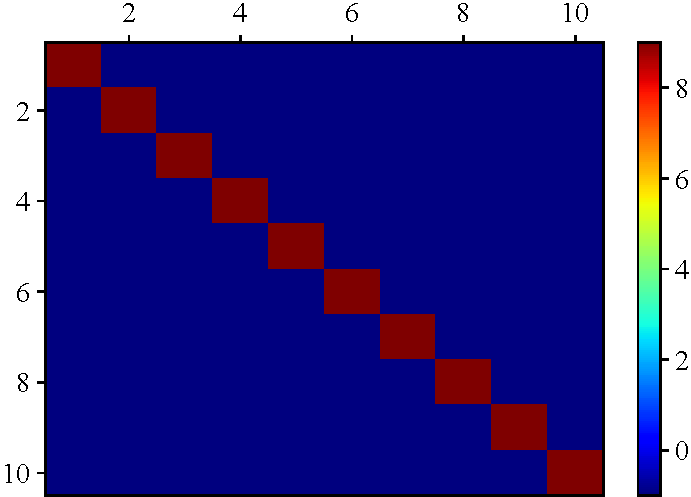
\includegraphics[width=.45\textwidth]{var_matrix_10.pdf}
    \label{fig:var_matrix_10}
  }
  \subfloat[]{
    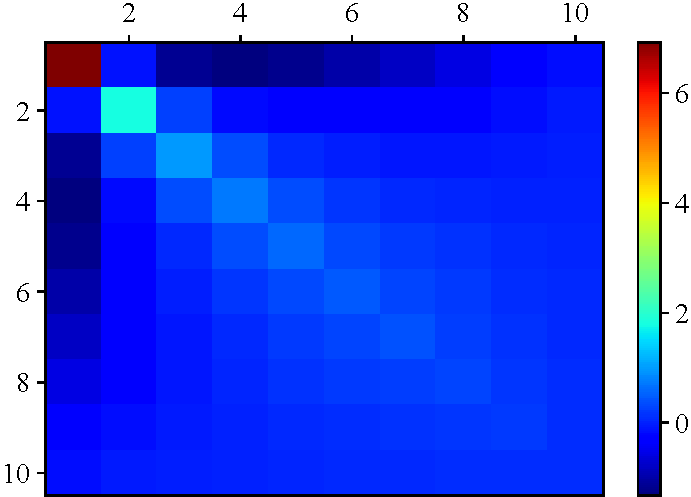
\includegraphics[width=.45\textwidth]{var_matrix_means_10.pdf}
    \label{fig:var_matrix_means_10}
  }
  \caption{(a) Variance matrix of samples for $n=10$; (b) Variance matrix of stepwise sample means for $n=10$.}
  \label{fig:var_10}
\end{figure}

\begin{figure}[!t]
  \centering
  \subfloat[]{
    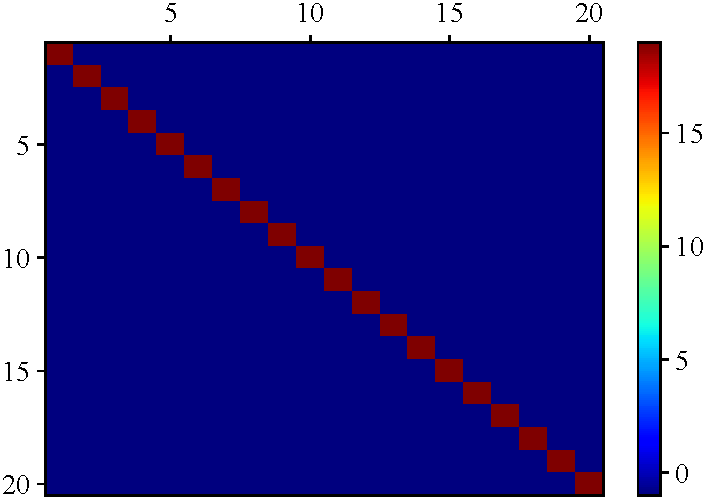
\includegraphics[width=.45\textwidth]{var_matrix_20.pdf}
    \label{fig:var_matrix_20}
  }
  \subfloat[]{
    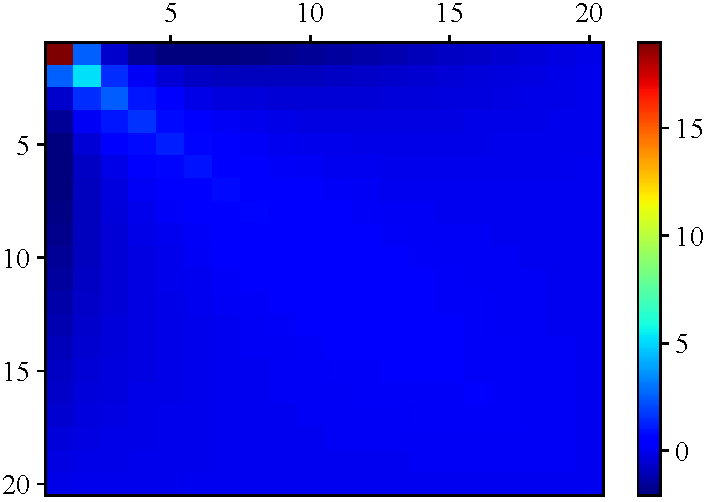
\includegraphics[width=.45\textwidth]{var_matrix_means_20.pdf}
    \label{fig:var_matrix_means_20}
  }
  \caption{(a) Variance matrix of samples for $n=20$; (b) Variance matrix of stepwise sample means for $n=20$.}
  \label{fig:var_20}
\end{figure}

\begin{figure}[!t]
  \centering
  \subfloat[]{
    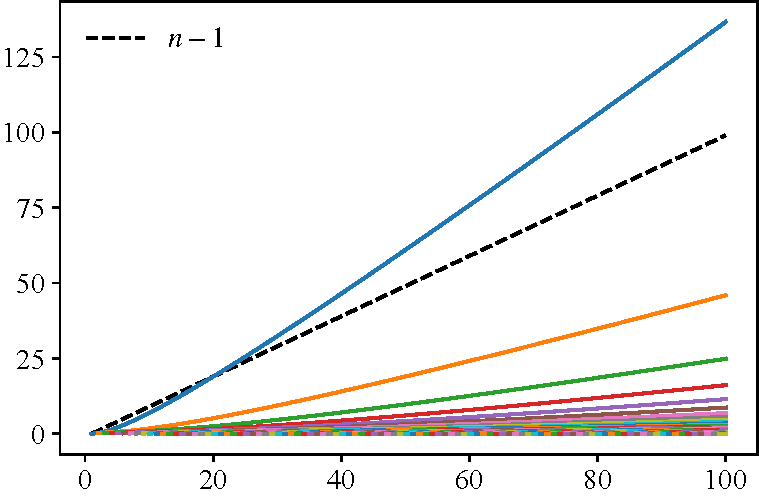
\includegraphics[width=.43\textwidth]{diag_var_matrix.pdf}
    \label{fig:diag_var_matrix}
  }
  \subfloat[]{
    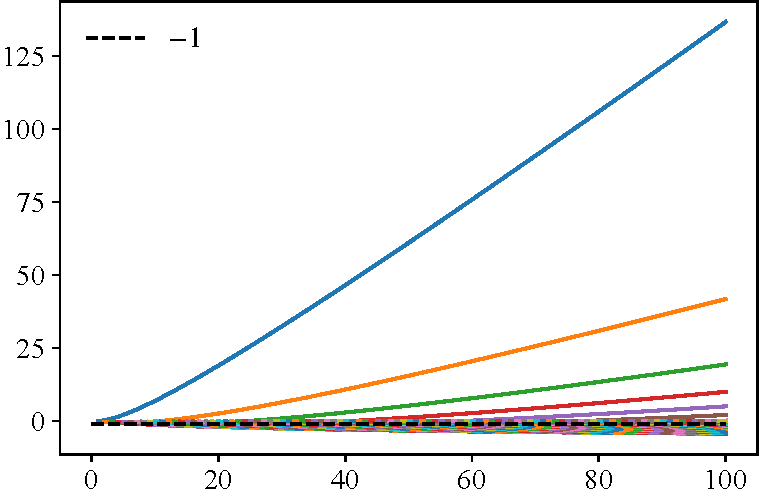
\includegraphics[width=.43\textwidth]{first_column_var_matrix.pdf}
    \label{fig:first_column_var_matrix}
  }
  \caption{(a) The diagonal elements of $\bar{V}$; (b) The first column of $\bar{V}$.}
  \label{fig:var_matrix_elements}
\end{figure}

As illustrations, the variance matrices of samples and stepwise sample means for $n=10$ and $n=20$ are shown in Fig.~\ref{fig:var_10} and Fig.~\ref{fig:var_20}, respectively. Furthermore, the diagonal elements and the first column of $\bar{V}$ with $n=1,2,\dots,100$ are presented in Fig.~\ref{fig:diag_var_matrix} and Fig.~\ref{fig:first_column_var_matrix}, respectively. It can be seen that $\bar{V}$ puts more weights to the front samples and less to the rear samples, while $V$ lays equal weights on each sample. Therefore, the arrangements of the samples make less difference on the variance of stepwise sample means than on the variance of samples. 

\begin{figure}[!h]
  \centering
  \subfloat[]{
    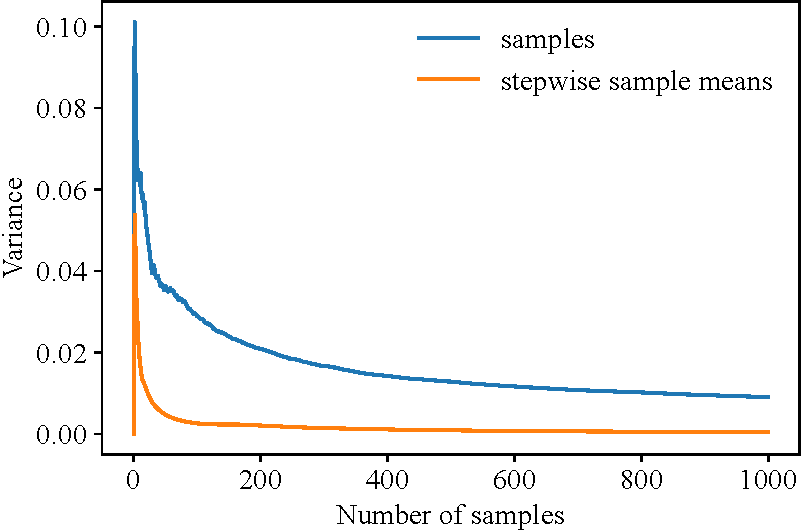
\includegraphics[width=.45\textwidth]{samples_vs_means_normal.pdf}
    \label{fig:samples_vs_means_normal}
  }
  \subfloat[]{
    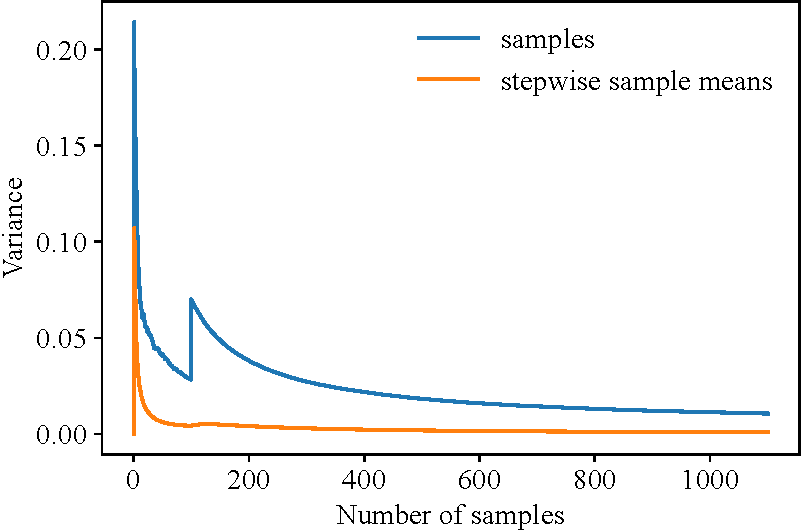
\includegraphics[width=.45\textwidth]{samples_vs_means_outlier.pdf}
    \label{fig:samples_vs_means_outlier}
  }
  \caption{(a) Variance of samples and stepwise sample means without outliers; (b) Variance of samples and stepwise sample means with an outlier.}
  \label{fig:var_samples_vs_means}
\end{figure}

For sample variance, the poor performance of some front samples will require many samples to mitigate. Specifically, a poor sample will bring huge variance at front, while can be ignored if in the rear. This phenomenon is demonstrated in Fig.~\ref{fig:var_samples_vs_means}, where an outlier is inserted as the $101^{\text{st}}$ sample. The outlier brings a sharp variance increase to the sample variance, while throwing no impact on the variance of stepwise sample means.

\end{document}
